\documentclass[journal]{IEEEtran}

\ifCLASSINFOpdf
\else
\fi

% correct bad hyphenation here
\usepackage[british]{babel}
\usepackage[hidelinks, unicode]{hyperref}
\usepackage[utf8]{inputenc}
\usepackage[T1]{fontenc}
\usepackage{amsmath}
\usepackage{bm}
\usepackage{amsfonts}
\usepackage{float}
\usepackage{array, booktabs, makecell}
\usepackage{xcolor}
\usepackage{comment}
\usepackage{lscape}
\usepackage{graphicx}

\usepackage[noabbrev,capitalize]{cleveref}

\begin{document}

\title{A Comparison between NEAT and Behavior Trees on OpenAI Gym Environments}
\author{
\href{https://github.com/fedeizzo}{Federico Izzo},
\href{https://github.com/francescobozzo}{Francesco Bozzo},
\href{https://github.com/BigEmperor26}{Michele Yin}
\\Department of Information Engineering and Computer Science\\University of Trento, Italy\\

\normalsize\{\href{mailto:federico.izzo@studenti.unitn.it}{\texttt{federico.izzo}}, 
\href{mailto:francesco-bozzo@studenti.unitn.it}{\texttt{francesco.bozzo}},
\href{mailto:michele.yin@studenti.unitn.it}{\texttt{michele.yin}}\} \texttt{@studenti.unitn.it}\vspace{-1em}}%

% make the title area
\maketitle

\begin{abstract}
This report presents a comparison between two evolution-based algorithms for solving control tasks on the OpenAI Gym framework: \textit{NeuroEvolution of Augmenting Topologies (NEAT)} and \textit{Behavior Trees (BT)}. Results show that while both algorithms are capable of obtaining decent results on simple tasks, NEAT often outperforms BT, although the latter offers more interpretability in debugging the agent's behavior.

Overall, this document provides insights into the strengths and weaknesses of these two popular algorithms and highlights the potential benefits of using them for tasks of different complexity.
\end{abstract}

\IEEEpeerreviewmaketitle

\section{Introduction}
\label{sec:intro}
This report presents a comparison between two evolution-based algorithms for solving control tasks on the OpenAI Gym environment: NEAT~\cite{NEAT} and BT~\cite{BT}. The former uses a genetic algorithm to evolve a topology, while the latter uses a hierarchical structure of decision-making nodes. The experiments were conducted on \textit{Frozen Lake}, \textit{Lunar Lander}, and \textit{Derk} environments supported by OpenAI's Gym.

\subsection{Frozen Lake}
Frozen Lake is a grid-world game that simulates an agent navigating through a frozen lake. The game is played on a grid of square tiles, where the agent starts at the top left cell and it must navigate through the frozen lake to reach the goal which is located on the other side of the map. At every step, the agent receives as input an absolute number that represents its position on the grid, and it can move in one direction.

The agent's goal is to reach the final tile without falling into any of the holes scattered around the environment; a positive reward (one) is provided only when the goal is reached before the time limit, otherwise the reward is zero. 

By default, the map has a fixed size of 4x4, but it can be also customized tweaking parameters. There is also the possibility to make the map slippery, therefore making the agent's moves non-deterministic.

\subsection{Lunar Lander}
Lunar Lander is a Gym environment that consists of a trajectory optimization problem in which a rocket has to land smoothly on a specific target pad area on the lunar surface. The observation space includes lander position, velocity, angle, angular velocity, and whether or not each leg is touching the ground.

There are three engines, two on the sides and one on the bottom of the rocket. Each engine can be activated individually to change the trajectory and velocity of the missile itself. Therefore the discrete action space is composed of the three engine fires and the do-nothing operation.

The reward function favors a lander that is moving slowly, near the landing pad, horizontally positioned, that can land safely on the ground while saving as much propellant as possible. According to its creators, agents that score more than 200 points are considered successful.

\subsection{Derk Gym}
Derk Gym is a MOBA-style \textit{Reinforcement Learning (RL)} environment shipped as an OpenAI Gym environment. The game has two teams in competition, and each of them is composed of three agents. The agent's goal is to defeat the enemy team and destroy the enemy tower by using up to three abilities that can consist of either offensive or defensive tools.

The environment is fully observable and there are a total of 64 pieces of information sensed from the environment. An agent can decide to move, rotate, focus, chase, and activate an ability. The reward function can be customized and it is computed based on players' interactions, for example encouraging damage to enemies and penalizing friendly fire. 

Derk Gym represents a challenging environment for many reasons, especially because some actions do not trigger an instant reward while others return zero feedback. Moreover, the interaction between agents is built on top of many variables, such as weapons and abilities.


\section{Methodologies}
\label{sec:methodologies}
In this project, we are considering two evolution-based techniques: NEAT and Behavior Trees.

\subsection{NEAT}
\textit{NeuroEvolution of Augmenting Topologies (NEAT)}~\cite{NEAT} is a technique for evolving arbitrary topologies like \textit{Neural Networks (NN)}. The goal is to obtain a NN capable of acting in a specific environment through the maximization of a given reward function. The learning process is driven by an \textit{Evolutionary Algorithm (EA)}, which tries to replicate the natural selection through the evolution of individuals inside a population, by using crossover and mutation.

A NN is created from a genome and each genome includes a list of connection genes, where a connection gene refers to two node genes. Additionally, each connection gene contains the weight that is used to represent the strength of the link between the two nodes.

To better explain how NEAT works, the following concepts are introduced: \emph{mutation}, \emph{crossover}, \emph{speciation}, and \emph{structural complexity}.

\subsubsection{Mutation}
Can occur to update the intensity of the connection gene or can modify the structure of the topology: a probability is associated to the creation/deletion of a new node/connection gene.

\subsubsection{Crossover}
During a run, a unique integer is associated with each new genome, in this way it is possible to create a complete hierarchical structure of the evolution of different NNs. This process is called \emph{historical marking}, and it is used in the core logic of the crossover algorithm.

\subsubsection{Speciation}
The population is divided into multiple species, and genomes compete against other individuals within the same species. This approach is used to overcome the phenomenon in which a new genome with a structural modification is removed from the population due to its low fitness value. The final goal is to stimulate structural mutations leaving enough time to assess the real performance of new individuals.

\subsubsection{Structural complexity}
\label{sec:structural-complexity}
NEAT tries to solve two optimization problems at the same time. The first one consists in the reward function optimization: given a topology we want to find the best possible set of weights that maximizes it. The second optimization task is related to the search of the best possible topology for the specific task. Due to the latter problem, the topology exploration can bring a complexity explosion: NEAT tries to avoid this by starting from small networks.

\subsection{Behavioural Trees}
A \emph{Behavior Tree (BT)} is defined as a tool to structure the switching between different tasks in an autonomous agent being both modular and reactive~\cite{BT}. As an alternative to Finite State Machines, they were first implemented to improve the behavior of Non-Player Characters (NPCs) in video games.

Due to the fact that there is no standard way to work with BTs, we decided to develop our own implementation to have full control over every detail from the design process, since many BTs are strictly linked with their target environments. Specifically, the BT library we devised includes:
\begin{itemize}
    \item implementation of action, condition, and composite nodes with memory.
    \item random initialization of BTs given a maximum height value;
    \item mutation and crossover strategies;
    \item simple evolution tools, such as elitism, size penalties, and pruning inactive nodes.
\end{itemize}
Each BT node can return a result and one of these three behavior states:
\begin{itemize}
    \item \texttt{SUCCESS} when a node has been successfully executed;
    \item \texttt{FAILURE} when a node has failed its execution;
    \item \texttt{RUNNING} when a time-consuming action is happening and the agent has to wait for some iterations to state whether it has been successful or not.
\end{itemize}

Since action and condition nodes are strictly connected to the target task solved by the BT, we implemented a different version of them for each OpenAI Gym environment we tested. Here it is presented a quick overview of different node types:

\subsubsection{Action Nodes}
The actual actions that the agent can perform through BTs are stored in action nodes.
In our implementation, each action has a duration that is defined as the number of environment iterations required to perform it. Action nodes do not return either \texttt{SUCCESS} or \texttt{FAILURE} until they have ended their execution: in that case, they yield the \texttt{RUNNING} state.

\subsubsection{Condition Nodes}
Condition nodes return boolean values while checking for some conditions on the input data that describe the environment with respect to some fixed constants.
For this reason, we implemented a good number of comparison operators that are commonly used in general-purpose programming languages: equal, greater, less, greater equal, less equal, and not equal. In all our experiments all the condition nodes return immediately either \texttt{SUCCESS} or \texttt{FAILURE} since they are applied on the agent's input observations.

\subsubsection{Composite Nodes}
Composite nodes are used to improve the logical information flow in BTs and they are the building block of any complex behavior that can be achieved with this framework. A composite node defines a list of children nodes that must be executed. There are two types of composite nodes:
\begin{itemize}
    \item \textit{sequence} nodes return \texttt{SUCCESS} if all children return \texttt{SUCCESS};
    \item \textit{fallback} nodes return \texttt{SUCCESS} if any children returns \texttt{SUCCESS}, otherwise \texttt{FAILURE} is propagated.
\end{itemize}
A BT can be viewed as a function that returns the action that maximizes the reward function given the environment state provided as input: each evaluation of it is called \texttt{tick} and the decision process is propagated from the root node to its sub-trees in a recursive way using a DFS-like strategy. The BT execution stops when leaves propagate either \texttt{FAILURE} or \texttt{SUCCESS} responses towards the tree root. If the state \texttt{RUNNING} is provided, the final result can be retrieved in the next ticks thanks to the memory implemented on composite and action nodes. 


\section{Results}
\label{sec:results}
\subsection{Frozen Lake}
As presented in \cref{sec:intro}, Frozen Lake is the simplest scenario we considered for evaluating our solutions.

\subsubsection{NEAT}
Since the only information that can be sensed from the environment is the agent position, the final agent is overfitted on the map that is used in the training procedure. When working with the deterministic version of the environment (not slippery), this constraint allowed us to stop the evolution process once having at least one maximized topology with fitness equal to one.

We opted for a fully-connected NN in which each node is connected to every other node of the previous and next layer: one input value for the agent position and four outputs for the possible actions. The performed action is chosen by running the \texttt{argmax} function on the four output nodes. Once a single topology with fitness equal to one is found, the evolution process is stopped, since the optimal agent has been achieved.

Interestingly, the evolution process was not converging when dealing with a single input with range \([0,15]\) (using the 4x4 map) to describe the agent position. Therefore, we decided to encode it through one-hot encoding, in order to limit input values in the range \([0,1]\). In this case, after one or two generations with population size of 200, the optimal topology is found on the 4x4 grid size.

When enabling the slippery option, on our experiments it is impossible to find an optimal agent which is able to solve the environment consistently, since the intended action is not always performed.

\subsubsection{BT}
Also when using Behavior Trees, the agent is overfitted on the specific grid composition. Even though by looking at \cref{fig:fitness-bt-frozen-lake} it looks like that the maximum fitness value is never fully achieved, this happens because BTs can be penalized of a multiplicative factor (in this case \(0.01\)) on the number of nodes and tree depth. This prevents the exponential increase of the size that could occur as a result of recombination.

\begin{figure}
    \centering
    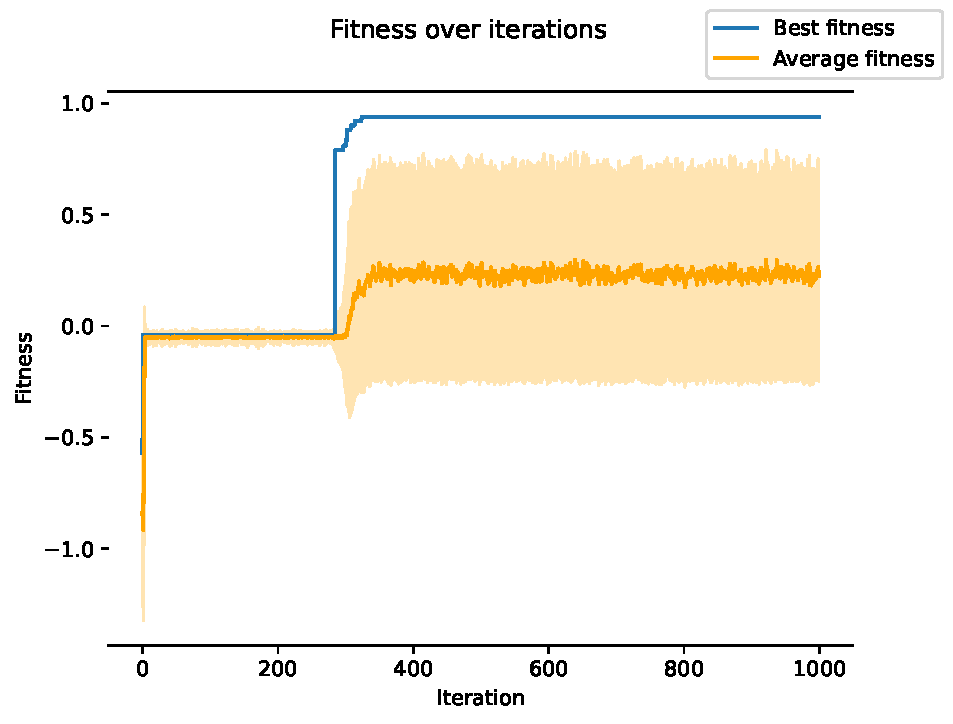
\includegraphics[width=0.8\linewidth]{./images/fitness_over_iterations_frozenlake_bt.pdf}
    \caption{Best and average fitness over iterations on Frozen Lake BT with std represented by the light orange area.}
    \label{fig:fitness-bt-frozen-lake}
\end{figure}

\subsection{Lunar Lander}
Lunar Lander is more complex with respect to Frozen Lake due to the increased number of variables involved. Results in this environment turned out to be not consistent since the fitness function receives a huge bump of 100 points when successfully landing in the pad.

\subsubsection{NEAT}
In this case, using the same Frozen Lake configuration NEAT is able to obtain good results as shown in \cref{fig:fitness-neat-lunar-lander}. Moreover, to make the final agent more stable, the score of an agent is computed by averaging the evaluation over five runs with different random seeds.

\begin{figure}
    \centering
    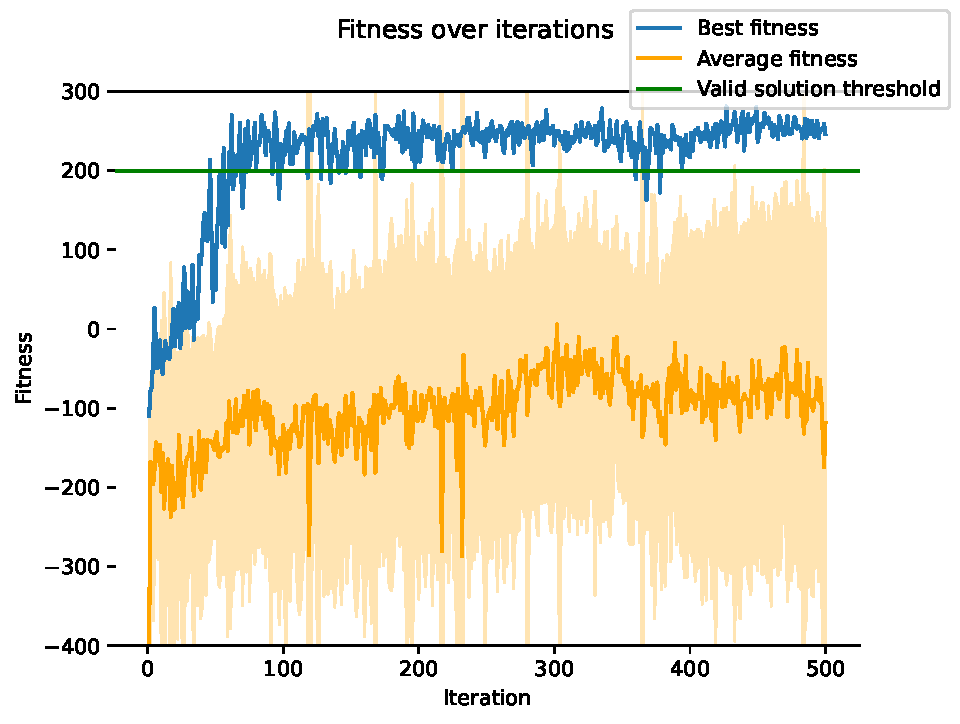
\includegraphics[width=0.8\linewidth]{./images/fitness_over_iterations_lunar_lander_neat.pdf}
    \caption{Best and average fitness over iterations on Lunar Lander NEAT with std represented by the light orange area.}
    \label{fig:fitness-neat-lunar-lander}
\end{figure}

\subsubsection{BT}
Similarly to NEAT, we started from the configuration used in Frozen Lake. In this case, in \cref{fig:fitness-bt-lunar-lander} we tested the environment with a single random seed, that influences the map creation and the initial inertia of the spaceship.

We noticed that the tree obtained was bloated with hundreds of nodes. In order to reduce the number of nodes and at the same time improve interpretability of the model, we added a metric that punishes the size of BTs. Additionally, we started tracking the percentage of active nodes: we then used this information to prune inactive nodes with \(0.05\) probability. Such a small percentage is chosen to guarantee some initial exploration of the search space through recombination of unused BT branches before starting the exploitation process.

\begin{figure}
    \centering
    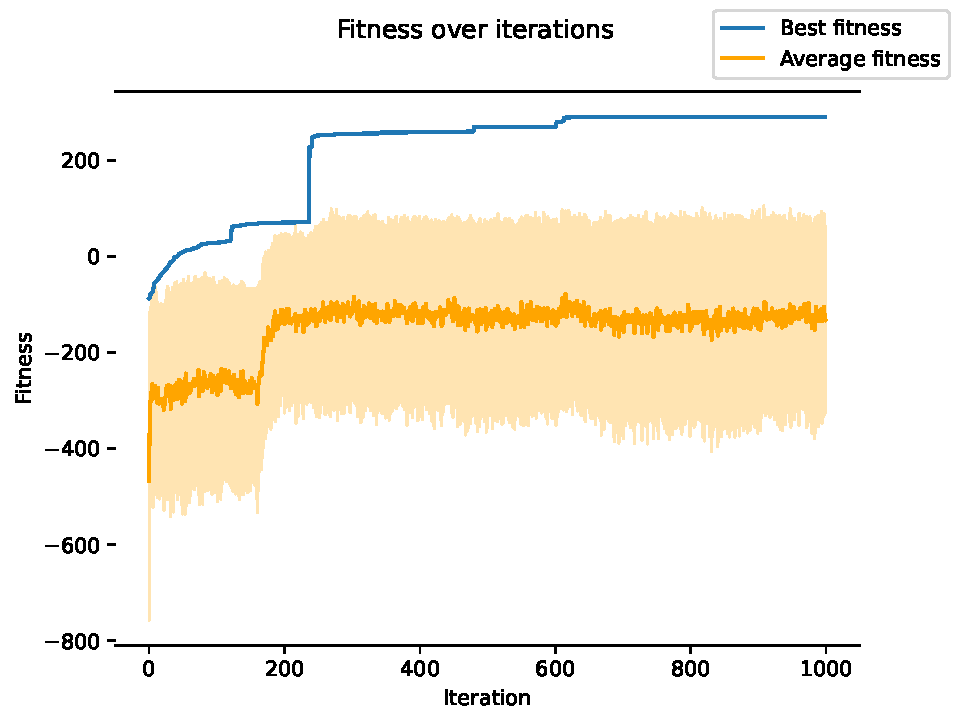
\includegraphics[width=0.8\linewidth]{./images/fitness_over_iterations_lunar_lander_bt.pdf}
    \caption{Best and average fitness over iterations on Lunar Lander BT with std represented by the light orange area.}
    \label{fig:fitness-bt-lunar-lander}
\end{figure}

However we noticed that the best BT is overfitted on the random seed used during the training phase and it is unable to land correctly with different initial conditions. We have tried to overcome this limitation by evaluating the fitness of a BT over different initial conditions (as we did in NEAT), but we found that this setup does not converge. This is could be a consequence of the fact that BT has a different evolution process with respect to NEAT since it does not cluster agents in species.

\subsection{Derk Gym}
Derk Gym is the most complex environment: we used it as a stretch goal to evaluate NEAT and our BT implementation.

\subsubsection{NEAT}
NEAT NNs receive as inputs from the environment 64 observation variables to produce 12 outputs, which grouped together enable the agent to move, rotate, chase, cast abilities, and focus targets: this configuration is called \texttt{64 input and 12 outputs}. Even though we performed extensive testings by tuning hyper parameters, the fitness scores showed an absence of an improving trend in the best fitness over subsequent generations, as can be seen in \cref{fig:fitness-neat-derk}. This could be related to the huge complexity of the search space and the consequential amount of time required for finding a potential optima.

% Therefore, as a second approach, we tried to reduce the input space only to the most important 13 variables. Additionally, we also modified the reward function to simplify the game dynamics. Unfortunately, the obtained results did not show an improvement and following this hypothesis we tried to shrink even more the problem size limiting the ability choice to only one item and removing the possibility of rotation and chase, this experiment was denominated \texttt{13 inputs and 10 outputs}.

Therefore, as a second approach, we tried to reduce the input space to the most important 13 variables and the output space by removing the possibility of rotation and chase. Additionally, we also modified the reward function to simplify the game dynamics and selected fixed abilities and weapons. We refer this experiment as \texttt{13 inputs and 10 outputs}. Unfortunately, also in this case the results were not promising.

\begin{figure}
    \centering
    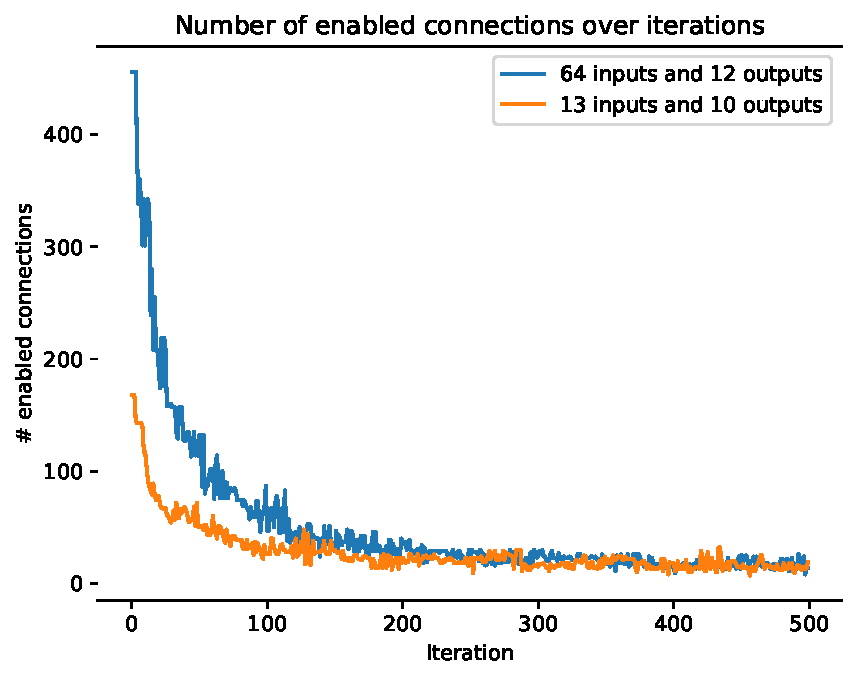
\includegraphics[width=0.8\linewidth]{./images/n_enabled_connections_over_iterations_derk_neat.pdf}
    \caption{Number of best network enabled connections over iteration Derk environment with NEAT solver.}
    \label{fig:enabled-connection-iteration-derk-neat}
\end{figure}

While investigating, we noticed that the number of enabled connections exponentially decreases over generations, as can be observed in \cref{fig:enabled-connection-iteration-derk-neat}. 
Since there is no correlation between the number of enabled connections and the number of nodes or the fitness value, we attributed the exponential decrease to the sparsity of the initial population. As already presented in \cref{sec:structural-complexity}, due to the dual optimization problem addressed during the NEAT evolution process, it would be better to start the evolution from simple structures. Therefore we simplified the initial topologies reducing the number of hidden layers and choosing different initial connection strategies, but the outcome was almost indistinguishable.

By looking at Reinforcement Learning state-of-the-art solutions, we then moved to a different approach based on Q-learning~\cite{DEEPQL}, in which each output node represents a single possible action that can be taken by an agent. In this case, the action space is composed of almost $1000$ possible actions obtained by linearly sampling the output space: a topology that requires so many output nodes should also have a deep structure. The increased size of topologies brought to the already known explosion of complexity: even with this attempt there was no visible improving trend over generations in terms of best fitness.

Alternatively, we attempted to reduce the action space to a limited set of 25 pre-computed actions, with the goal of simplify as much as possible the Q-learning problem. This last approach did not work as well, as presented in \cref{fig:fitness-neat-derk}.

% TODO: perche' il 25 action non funziona come dovuto e ha best fitness sempre vicina a zero?

\subsubsection{BT}
Also with BTs, we tested different evolutionary algorithms varying different hyper parameters and reducing the evolution space, but we quickly realized that all approaches were failing similarly to NEAT, as shown in \cref{fig:fitness-bt-derk}.

\begin{figure}
    \centering
    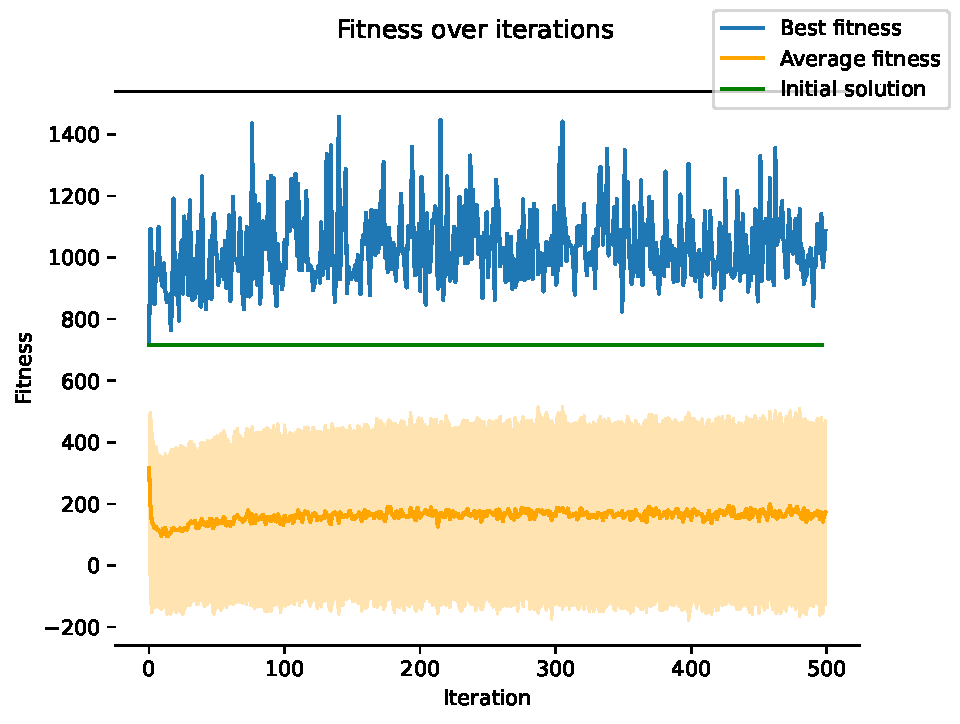
\includegraphics[width=0.8\linewidth]{./images/fitness_over_iterations_derk_bt.pdf}
    \caption{Best and average fitness over iterations on Derk BT with std represented by the light orange area.}
    \label{fig:fitness-bt-derk}
\end{figure}

Since BTs are intepretable, we have tried handcrafting simple BTs testing different tree topologies. This helped us in debugging the environment and discover that some actions may return no feedback: for example the gun does not shoot if the target is not in a certain range. This lack of feedback is a crucial missing step on modelling complex behaviors with BTs, since action nodes should be able to return whether the action succeeded or not.

In addition to this, we also discovered that some actions may take many environment steps to be fully performed: for example a bullet takes time to reach the enemy which depends on the distance.
This implies that the instantaneous agent reward is not always related to action just performed, but also to some past actions.

Moreover, we handcrafted a BT that chases enemies and their tower if not in range, shoots at them until their HP is down to 0. Then we tried to initialize the BT evolution process with this tree, but after some generations the outcomes were similar to the ones with random initialization.


\section{Conclusion}
\label{sec:conclusion}
% - What difficulties were encountered during the project (if any), and what steps were taken to overcome those difficulties?
% - A discussion of the lessons learned from the project.
% - What conclusions can be drawn from the work? 

As presented previously, to obtain some decent results on complex environments, many different approaches have been implemented to tackle the issues we faced: agent robustness on environment changes (random seed, environment variables) and environment complexity. Many of our attempted workarounds have been inspired by state-of-the-art solutions from other applications, such as pruning and Q-learning. Alternatively, we also tried to simplify complex environments by reducing the number of variables, such as fixing weapons and abilities on Derk.

\Cref{tab:neat-vs-bt} summarizes NEAT and BT performances over the tested environments. While both techniques are able to reach the optimal agent on Frozen Lake, please consider that BTs on Lunar Lander have been evolved and tested only on a single random seed, therefore the table entry could be misleading. Moreover, NEAT outperforms BT in the Derk environment.

In general, BTs should be preferred with respect to NEAT when explainability is necessary, especially when keeping limited tree sizes thanks to pruning or penalization.

\begin{table}[t]
    \caption{NEAT and BT max fitness in different environments.}
    \begin{center}
        \begin{tabular}{lrr}
            \toprule
            Environment & NEAT & BT \\
            \midrule
            Frozen Lake  & 1    &  \(^* 0.94\) \\
            Lunar Lander & 281  & \(^* 291\) \\
            Derk         & 2038 & 1087 \\
            \bottomrule
        \end{tabular}
    \end{center}
    \label{tab:neat-vs-bt}
\end{table}

\section{Contributions}
\label{sec:contributions}
\begin{itemize}
    \item Federico Izzo: worked mainly on the NEAT development;
    \item Francesco Bozzo: BT and NEAT support.
    \item Michele Yin: worked mainly on the BT development;
\end{itemize}

Most of the initial work regarding NEAT and especially Behavior Trees was also developed by our former team member Samuele Conti.

Please, consider that the GitHub contributor section does not represent the actual statistic to measure the personal work of each member, since from time to time we worked together on a single laptop or we uploaded run logs.



\bibliography{bibliography.bib}{}
\bibliographystyle{IEEEtran}

\clearpage
\newpage
\onecolumn
\appendices
\section{Figures and Tables}

\begin{figure}[H]
    \centering
    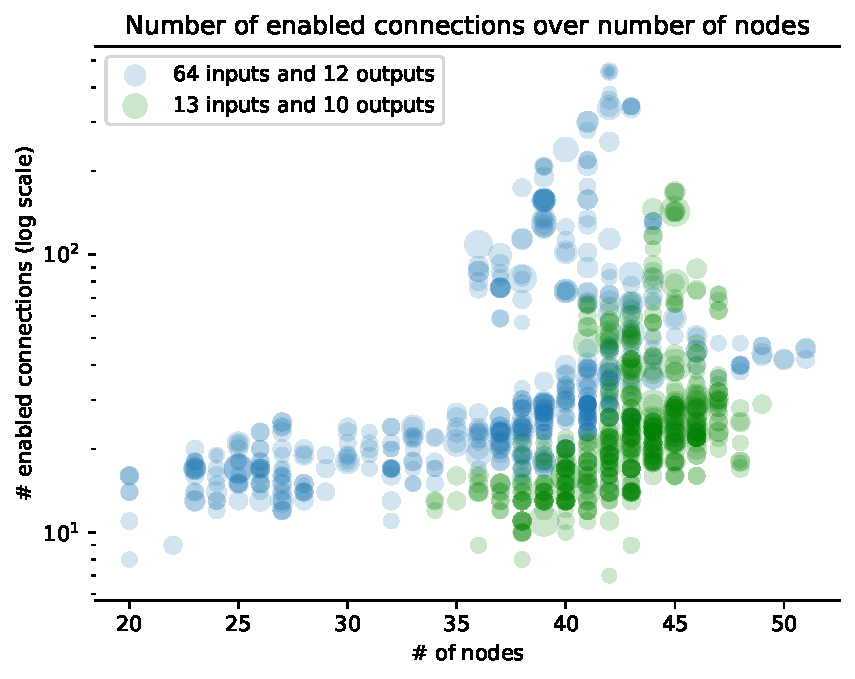
\includegraphics[width=0.6\linewidth]{./images/n_enabled_connections_over_n_nodes_derk_neat.pdf}
    \caption{Number of enabled connections (in logarithmic scale) over number of nodes of a NEAT solver on Derk environment for the best network at each generation. The size of scatters represents the fitness value of the agent. No emerging pattern can be noticed between the decrease of enabled connections over time and the number of nodes.}
    \label{fig:enabled-connection-nodes-derk-neat}
\end{figure}

\begin{figure}[H]
    \centering
    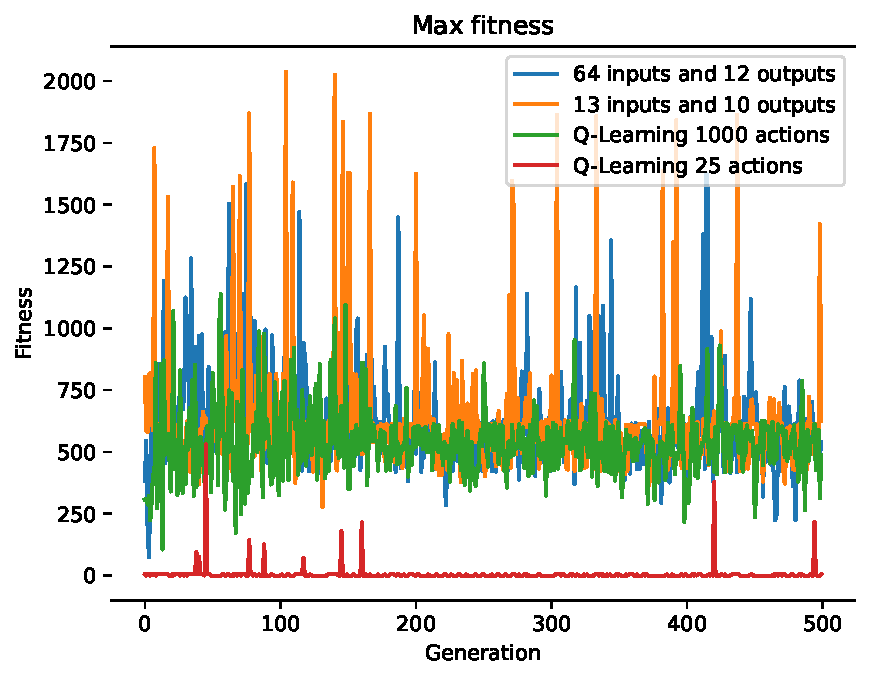
\includegraphics[width=0.6\linewidth]{./images/fitness_over_iterations_derk_neat.pdf}
    \caption{Best fitness over generations on different NEAT attempts on the Derk environment, low performances of the Q-learning 25 actions are a consequence of the different range of the abilities and the low probability of moving enough close to enemies.}
    \label{fig:fitness-neat-derk}
\end{figure}



% \begin{table*}
%     \caption{BT node output}
%     \begin{center}
%         \begin{tabular}{lccc}
%             \toprule
%             Node type & Succeeds & Fails & Running \\
%             \midrule
%             Fallback & If one child succeeds & If all children fail & If one child returns Running \\
%             Sequence & If all children succeed & If one child fails & If one child returns Running \\
%             Action & Upon completion & Impossible to complete & During completion \\
%             Condition & If true & If false & Never \\
%             \bottomrule
%         \end{tabular}
%     \end{center}
%     \label{tab:bt-node-output}
% \end{table*}

\begin{table*}
    \caption{Performance summary}
    \begin{center}
        \begin{tabular}{llrrrr}
        \toprule
        {}   &  Env & Generation &  Max fitness &        Mean &         Std \\
        Name &  &  &  &  &  \\
        \midrule
        BT          & Frozen Lake & 72 & 0.94 &  -0.0482 & 0.1347 \\
        NEAT        & Frozen Lake & 1 & 1 &  0.00500 & 0.07053 \\
        BT          & Lunar Lander & 654 &  291 &  -132.377  & 187.8  \\
        NEAT        & Lunar Lander & 500 &  281.036445 &  -85.143571 & 238.081605 \\
        BT          & Derk &  500 &  1086.568 & -172.413   & 298.638  \\
        64 inputs and 12 outputs & Derk & 414 & 1627.199951 &  -41.238786 & 461.072898 \\
        13 inputs and 10 outputs & Derk & 104 & 2038.612549 & -108.815655 & 713.525290 \\
        Q-Learning 1000 actions  & Derk &  56 & 1138.235474 & -122.275397 & 378.131604 \\
        Q-Learning 25 actions    & Derk &  45 &  530.440002 &    7.012384 & 101.492292 \\
        \bottomrule
        \end{tabular}
    \end{center}
    \label{tab:performance-summary}
\end{table*}


% \pagebreak
\begin{figure}
    \centering
    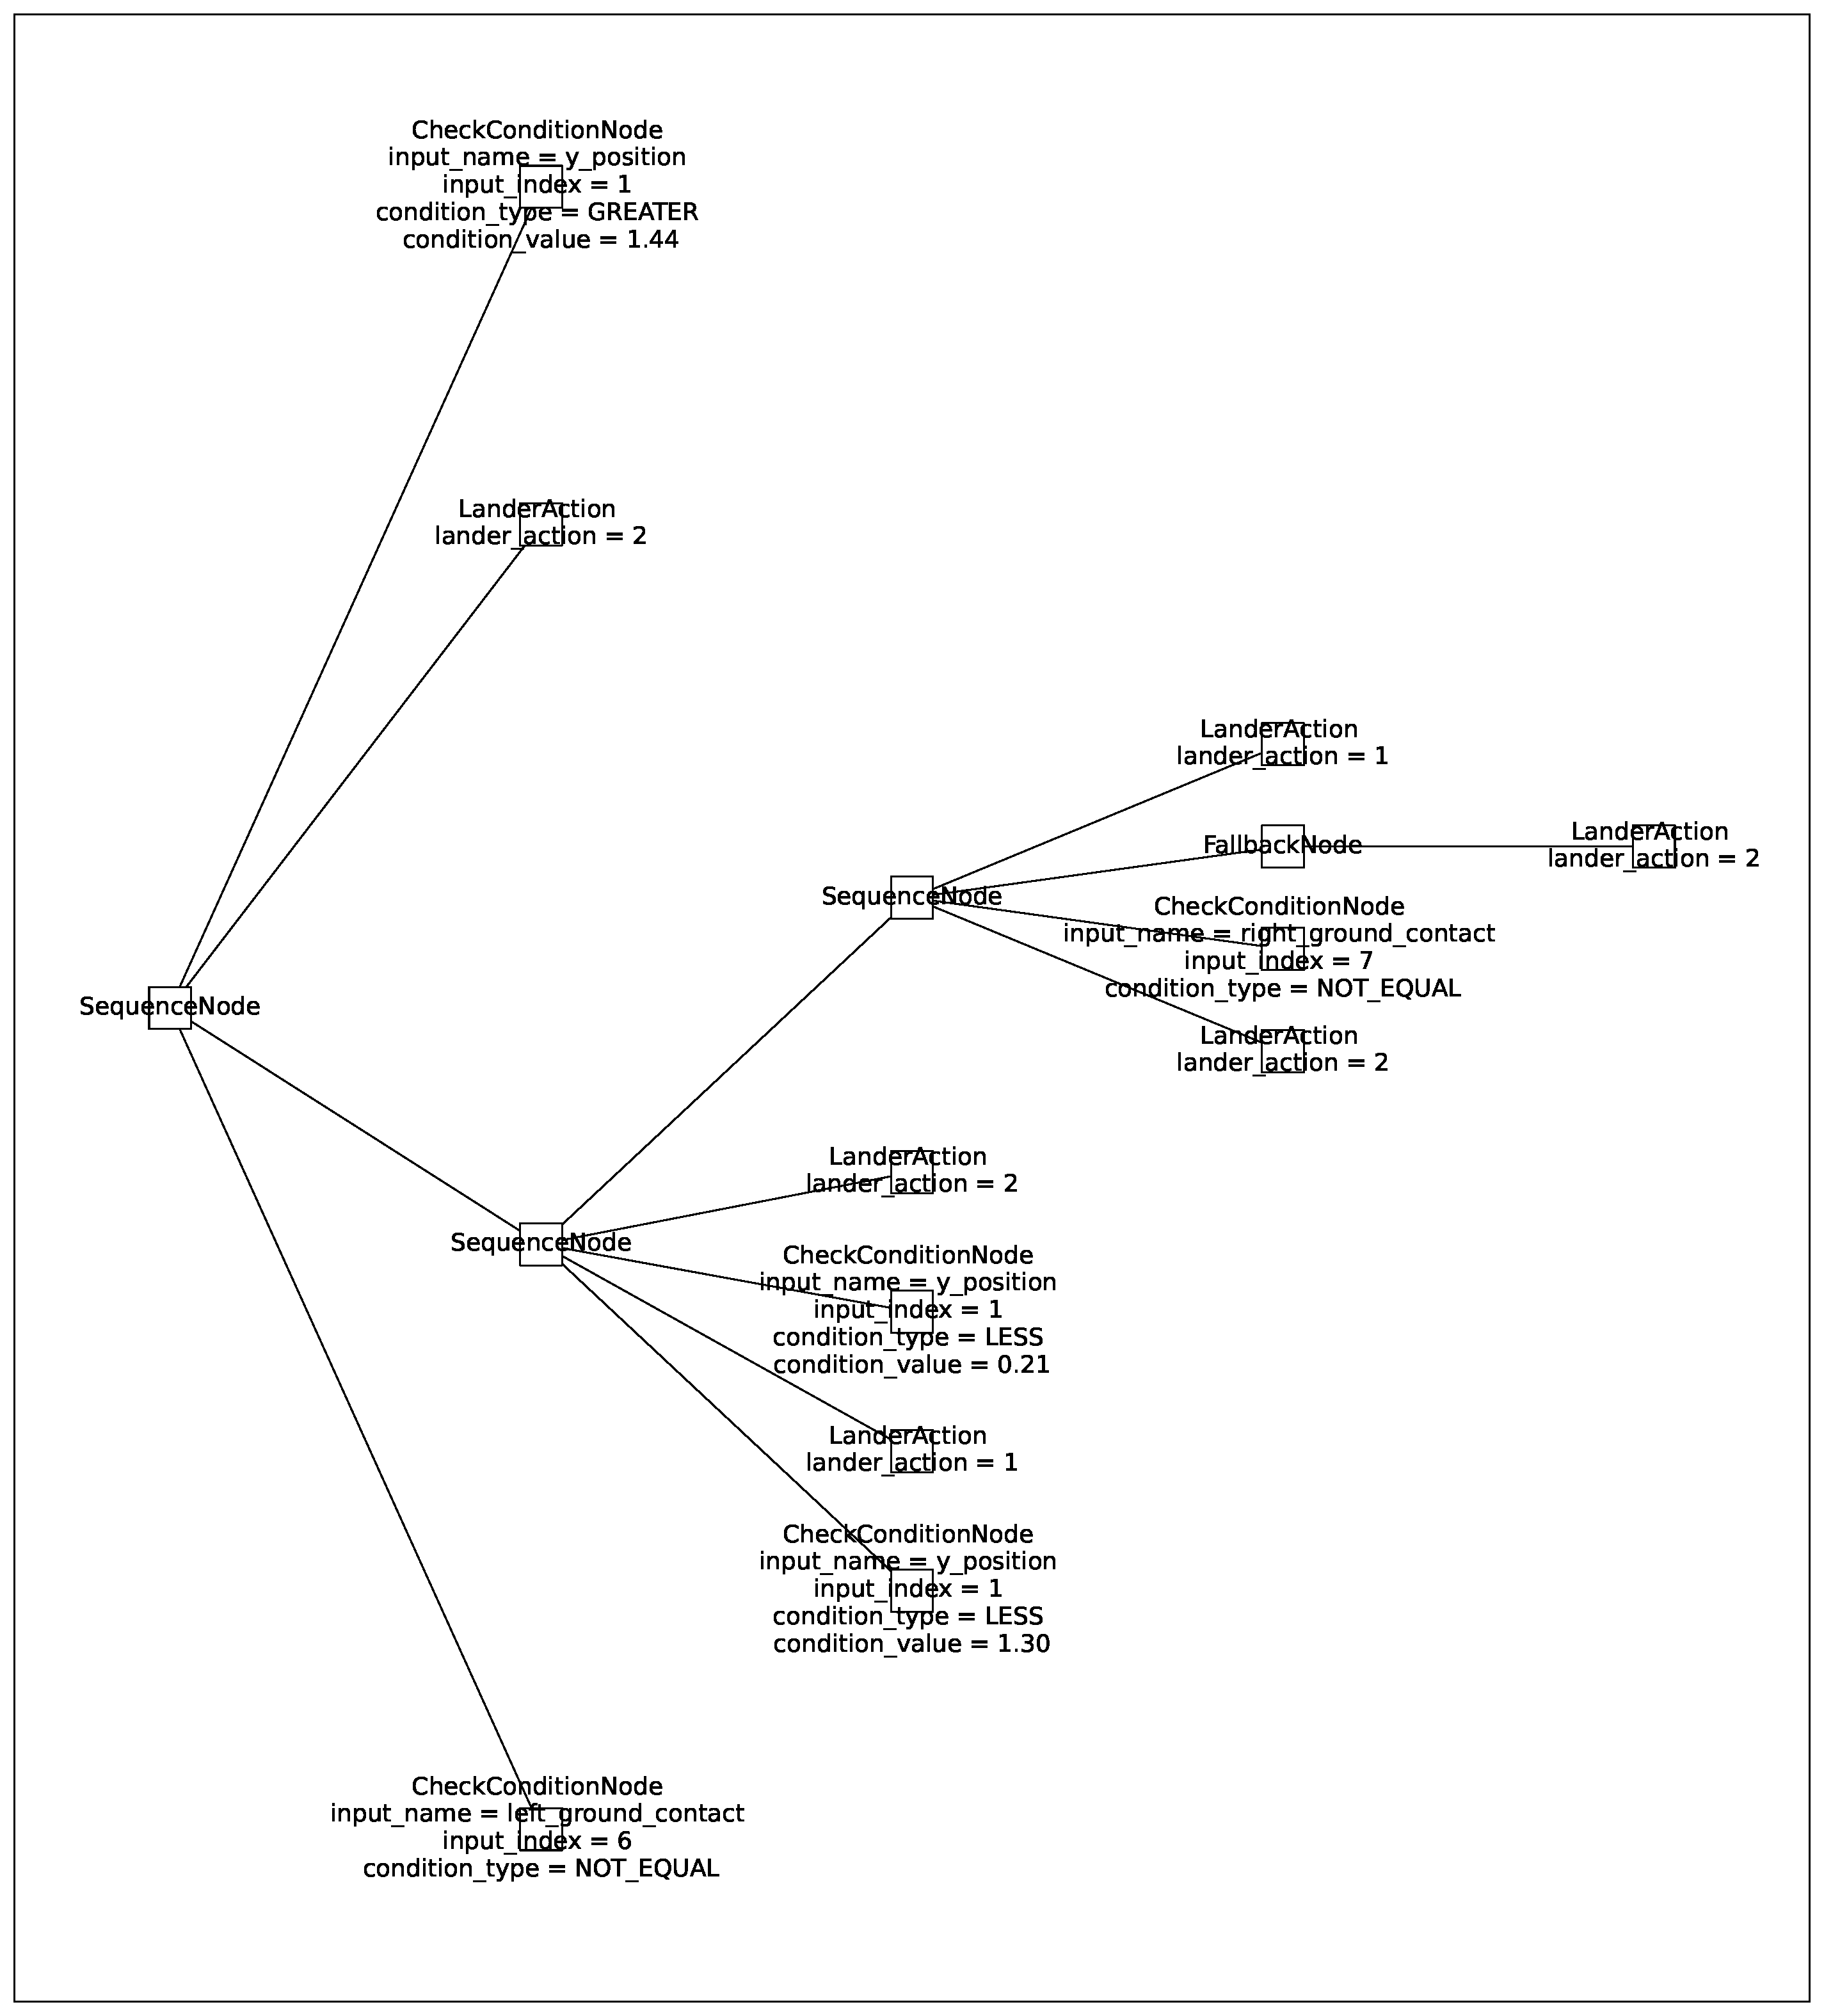
\includegraphics[width=1\linewidth]{./images/lander_BT.pdf}
    \caption{Visual representation of the best BT for Lunar Lander with the root as the leftmost node. The tree nodes are traversed from left to right and from bottom to top in a DFS-like fashion. We can see from the condition nodes that the Lander completely ignores every other input except its y position, which is probably one key element that prevents generalization of this tree on other random seeds. }
    \label{fig:lander-bt-figure}
\end{figure}

\end{document}
